\subsection{2DJ and PSYCHE}
\label{subsec:noah__2djpsyche}

So far, I have exclusively used the CLIP-COSY as the final homonuclear module in NOAH supersequences.
In general, since homonuclear modules are placed at the end of supersequences, there is rarely any need to adapt them for NOAH supersequences, as they do not need to preserve any magnetisation.
One exception to this is the family of 2DJ and pseudo-2D pure shift experiments, where the spectral width in the indirect dimension is extremely small, on the order of \qty{50}{\Hz}.
In such cases, the number of $t_1$ increments required is far smaller than for a typical 2D experiment.
Since---by default---each module in a NOAH supersequence is acquired with the same number of increments, directly concatenating such modules to the end of a supersequence would therefore prove suboptimal.

However, as described previously in \cref{subsec:noah__hmqc,subsec:noah__sehsqc_n}, it is possible to reduce the number of $t_1$ increments for a particular module, and in exchange, increase the number of scans recorded for that module.
In the context of \nitrogen{} modules, this was a `special' procedure referred to as $k$-scaling; however, for these homonuclear modules, it is natural and necessary.
One difference in the implementation is that, instead of specifying a value $k$ by which \texttt{TD1} is scaled down and \texttt{NS} scaled up, the user is allowed to directly specify the number of $t_1$ increments as an integer (\texttt{CNST37} in TopSpin).
This value must be a divisor of the \textit{normal} number of $t_1$ increments for all other modules (or equivalently, $k$ must be an integer).
The `indirect-dimension spectral width' is specified as \texttt{CNST38}: for pure shift modules this quantity is more properly referred to as the reciprocal of the chunk size, i.e.\ $1/\Tchunk$.

\begin{figure}[!ht]
    \centering
    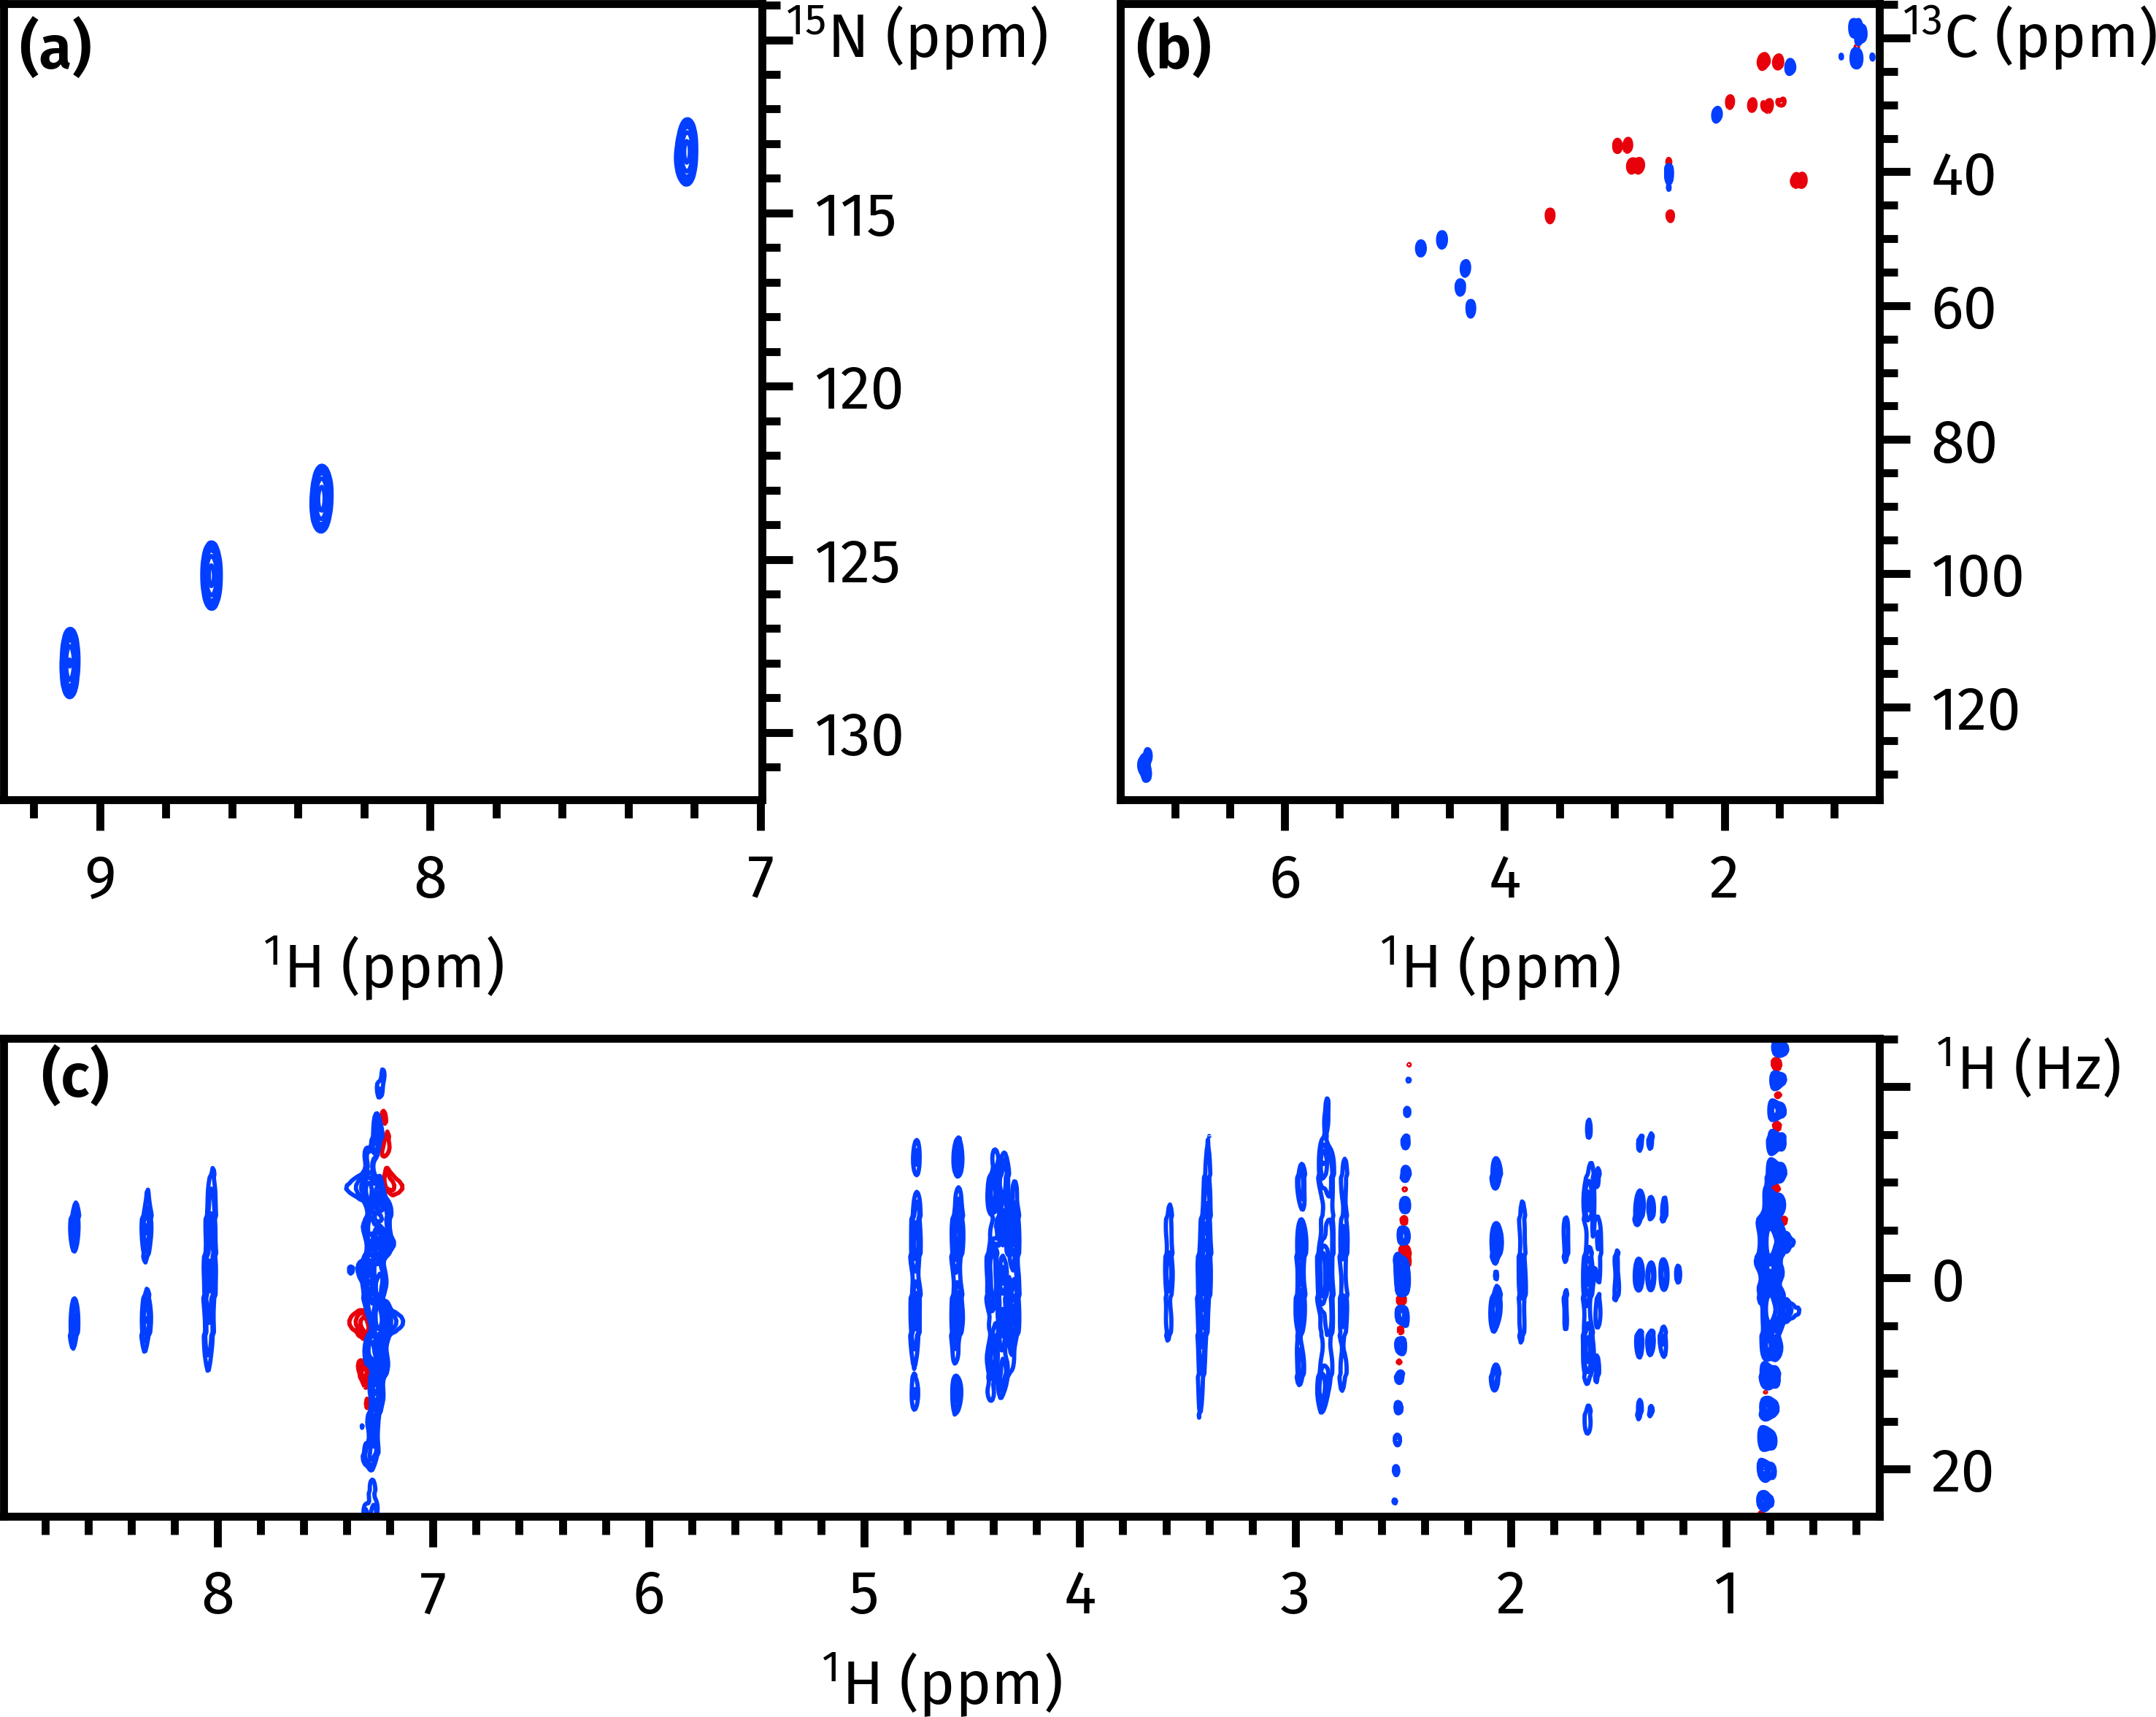
\includegraphics[]{noah/2dj_example.png}%
    {\phantomsubcaption\label{fig:2dj_example_spn}}%
    {\phantomsubcaption\label{fig:2dj_example_spc}}%
    {\phantomsubcaption\label{fig:2dj_example_j}}%
    \caption[Spectra from a \noah{Spn,Sp,J} supersequence]{
        Spectra obtained from a \noah{Spn,Sp,J} supersequence.
        \textbf{(\subref*{fig:2dj_example_spn})} \nitrogen{} seHSQC (128 $t_1$ increments and 2 scans per increment).
        \textbf{(\subref*{fig:2dj_example_spc})} \carbon{} seHSQC (128 $t_1$ increments and 2 scans per increment).
        \textbf{(\subref*{fig:2dj_example_j})} PSYCHE 2DJ (32 $t_1$ increments and 8 scans per increment).
        \datacode{7G-201028}
    }
    \label{fig:2dj_example}
\end{figure}

The modules thus implemented include the standard magnitude-mode 2DJ experiment, the PSYCHE 2DJ experiment\autocite{Foroozandeh2015CC}, the original 1D PSYCHE\autocite{Foroozandeh2014ACIE}, and the 1D TSE-PSYCHE\autocite{Foroozandeh2015CC}.
An example of the data thus obtained (with the PSYCHE 2DJ) is shown in \cref{fig:2dj_example}.
One particular advantage of including PSYCHE-type modules in NOAH supersequences is that sensitivity is not likely to be at a premium: this is partly because of the increased number of scans, but also partly because other 2D experiments have comparably low sensitivity (meaning that in the time needed to acquire an HSQC, for example, the PSYCHE experiment will also have sufficient sensitivity).
This allows the user to choose a relatively small flip angle (ca.\ \ang{10}) for the PSYCHE saltire pulses in order to minimise artefacts from imperfect decoupling (see also \cref{subsec:pureshift__psyche_analysis}).

\begin{figure}[!ht]
    \centering
    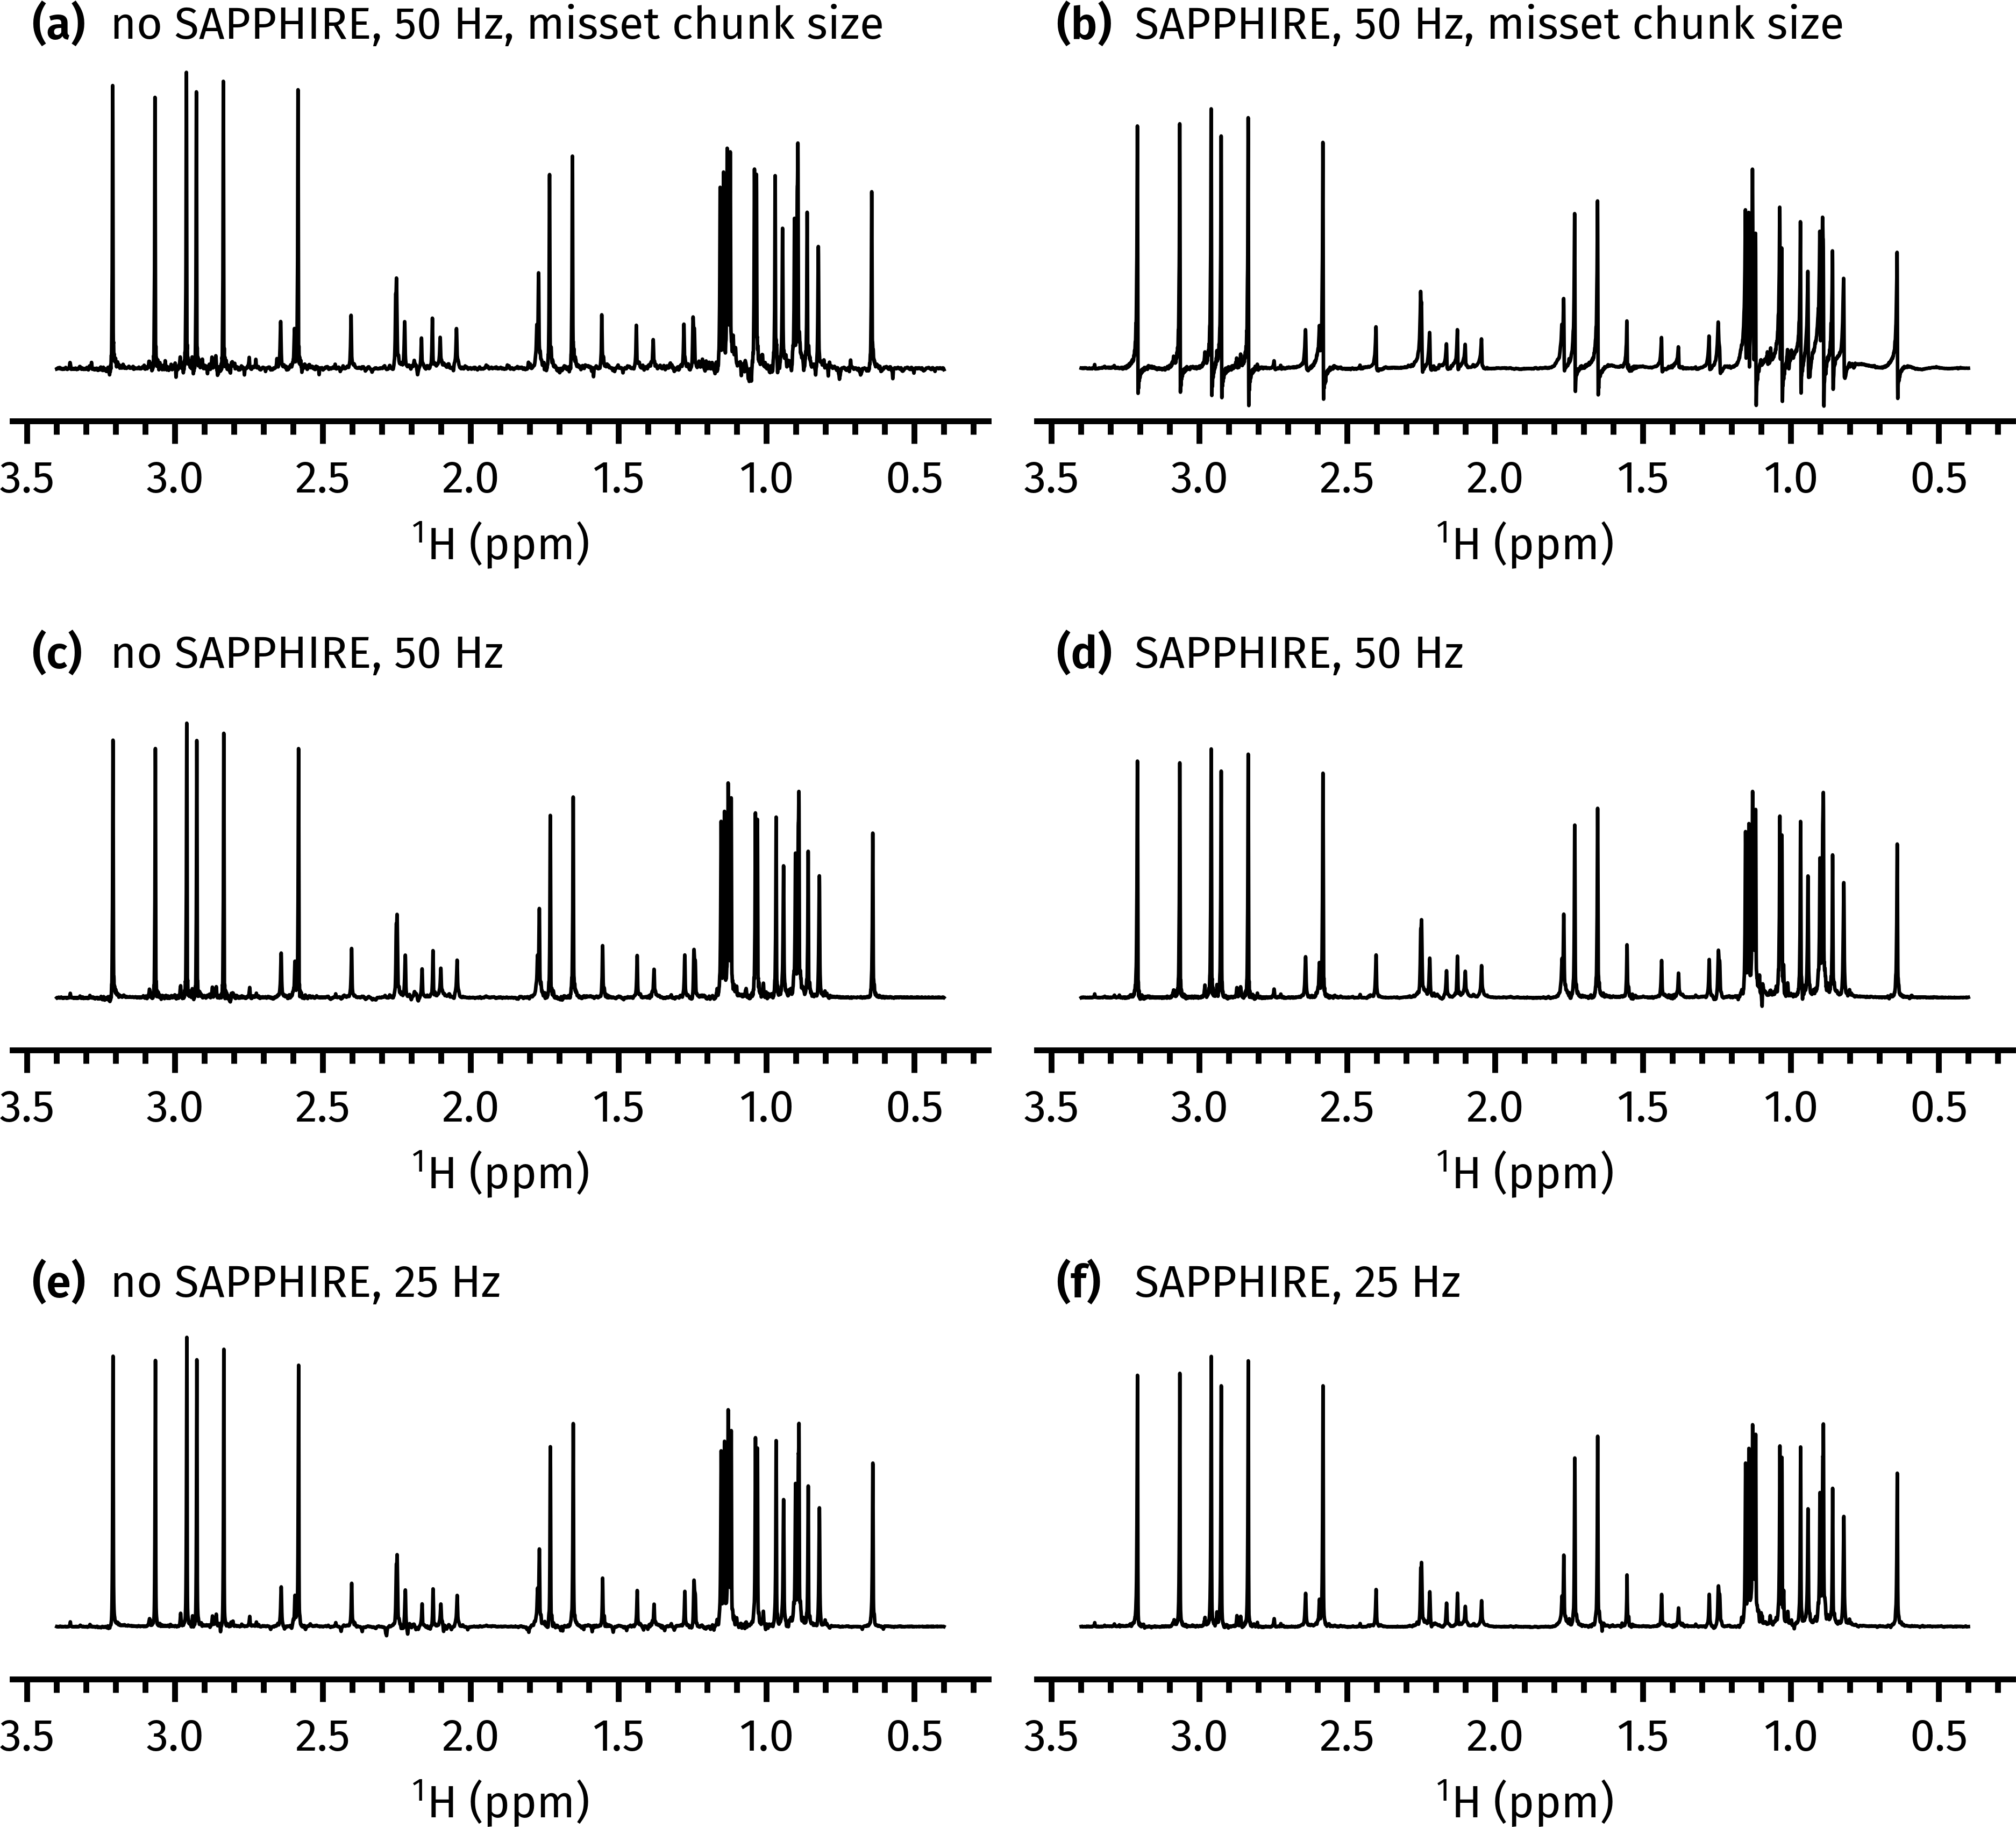
\includegraphics[]{noah/psyche_wrongsw1.png}%
    {\phantomsubcaption\label{fig:psyche_wrongsw1_bad_nosap}}%
    {\phantomsubcaption\label{fig:psyche_wrongsw1_bad_sap}}%
    {\phantomsubcaption\label{fig:psyche_wrongsw1_good_nosap}}%
    {\phantomsubcaption\label{fig:psyche_wrongsw1_good_sap}}%
    {\phantomsubcaption\label{fig:psyche_wrongsw1_good_nosap_25}}%
    {\phantomsubcaption\label{fig:psyche_wrongsw1_good_sap_25}}%
    \caption[Effect of automatic chunk size calculation and SAPPHIRE averaging on NOAH PSYCHE spectra]{
        A series of 1D PSYCHE spectra obtained from the \noah{Spn,Sp,P} supersequence (saltire flip angle of \ang{15}).
        \textbf{(\subref*{fig:psyche_wrongsw1_bad_nosap})} 1D PSYCHE spectrum acquired without SAPPHIRE averaging, and an incorrect chunk size which is not an integral number of complex data points. The `indirect-dimension spectral width' (more precisely, $1/\Tchunk$) is \qty{50}{\Hz}.
        \textbf{(\subref*{fig:psyche_wrongsw1_bad_sap})} 1D PSYCHE spectrum with  8-step SAPPHIRE averaging and an incorrect chunk size; this manifests as phase errors which cannot be corrected.
        \textbf{(\subref*{fig:psyche_wrongsw1_good_nosap})--(\subref*{fig:psyche_wrongsw1_good_sap})} The same as (\subref*{fig:psyche_wrongsw1_bad_nosap}) and (\subref*{fig:psyche_wrongsw1_bad_sap}), but with the chunk size automatically rounded in the pulse programme.
        \textbf{(\subref*{fig:psyche_wrongsw1_good_nosap_25})--(\subref*{fig:psyche_wrongsw1_good_sap_25})} The same as (\subref*{fig:psyche_wrongsw1_good_nosap}) and (\subref*{fig:psyche_wrongsw1_good_sap}), but with double the chunk size.
        This leads to a more striking difference between the data acquired without and with SAPPHIRE, as discussed in the original paper\autocite{Moutzouri2017CC}.
        \datacode{7C-211123}
    }
    \label{fig:psyche_wrongsw1}
\end{figure}

On top of this, for the 1D (TSE-)PSYCHE sequences, the extra transients can be used to perform SAPPHIRE averaging\autocite{Moutzouri2017CC}.
Ordinarily, the PSYCHE pulse sequence seeks to refocus J-couplings in the middle of each chunk (of duration $\Tchunk$).
This is accomplished through the \textit{prefocusing} of J-couplings in a spin echo of total duration $\Tchunk/2$.\autocite{Aguilar2010ACIE}
In the SAPPHIRE procedure, each chunk of the pure shift interferogram is instead collected several times, all while varying the exact point in time where J-coupling is perfectly refocused.
Summation of these data leads to the suppression of artefacts which arise due to the periodic J-modulation in the interferogram.
This averaging is somewhat analogous to a phase cycle, and performing an 8-step SAPPHIRE averaging procedure (for example) would often require the experiment to be lengthened beyond the duration which is truly necessary.
However, in the context of NOAH, since each chunk is acquired at least $k$ times, a $k$-step SAPPHIRE procedure can be incorporated `for free'.
In the GENESIS pulse programmes, this feature is enabled by default, although it can be turned off in developer mode where non-SAPPHIRE pure shift modules are available.

A final and more prosaic implementation detail is that in the 1D pure shift modules, the chunk size $\Tchunk$ is automatically rounded to the nearest even multiple of the dwell time $\tau_{\symup{dw}}$ (\texttt{DW} in TopSpin).
This ensures that each chunk consists of an integral number of complex data points.
Although this can be set by the user manually, it is very easy to forget, especially for someone not fully acquainted with the experiment; the results can be quite different, as illustrated in \cref{fig:psyche_wrongsw1}.
When an $n$-step SAPPHIRE averaging is used, the requirement is even stricter: $\Tchunk$ must be a multiple of $2n \tau_{\symup{dw}}$.
This is also encoded in the pulse programmes.
